\documentclass[tikz]{standalone}
\usepackage[utf8]{inputenc}
\usetikzlibrary{calc,intersections}

\definecolor{DarkRed}{rgb}{0.7,0.2,0.2}

\begin{document}

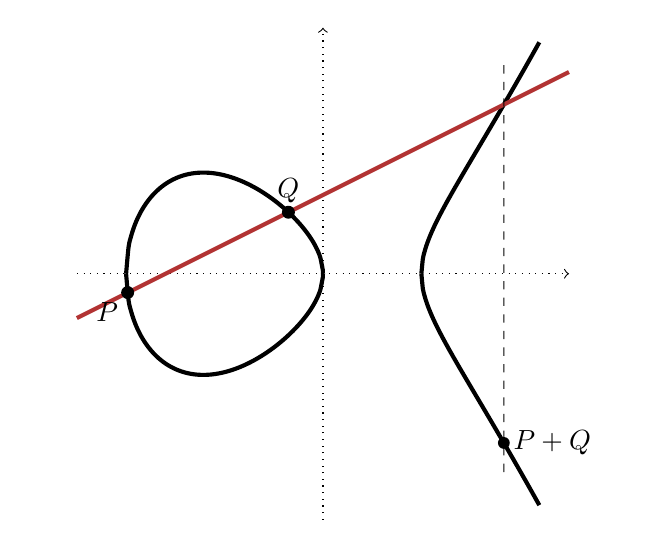
\begin{tikzpicture}[scale=2.5]
\def\ptsize{.03}
\clip (-1.5,-1.25) rectangle (1.5,1.25);
\draw[->,dotted] (-1.25,0) -- (1.25,0);
\draw[->,dotted] (0,-1.25) -- (0,1.25);
\path[domain=-1:0,smooth,samples=80,line width=1.5pt,name path=patatedessus,draw] plot (\x, {sqrt(\x^3 + .5*(\x)^2 - .5*\x)}) -- (0,0);
\path[domain=-1:0,smooth,samples=80,line width=1.5pt,name path=patatedessous,draw] plot (\x, {-sqrt(\x^3 + .5*(\x)^2 - .5*\x)}) -- (0,0);
\path[domain=.5:1.1,smooth,samples=80,line width=1.5pt,name path=branchedessus,draw] plot (\x, {sqrt(\x^3 + .5*(\x)^2 - .5*\x)});
\path[domain=.5:1.1,smooth,samples=80,line width=1.5pt,name path=branchedessous,draw] plot (\x, {-sqrt(\x^3 + .5*(\x)^2 - .5*\x)});

\path[DarkRed,domain=-1.25:1.25, name path=linePQ,line width=1.5pt,draw] plot (\x, {0.5*\x + 0.4});
\draw[name intersections={of=patatedessous and linePQ, by=P},fill] (P) circle (\ptsize);
\draw[name intersections={of=patatedessus and linePQ, by=Q},fill] (Q) circle (\ptsize);
\path[name intersections={of=branchedessus and linePQ, by=R},fill];
\path let \p1 = (R) in node (S) at (\x1,-\y1) {};
\fill (S) circle (\ptsize);
\draw[dashed,shorten >= -.5cm,shorten <= -.5cm] (R) -- (S);
\node[below left] at (P) {$P$};
\node[above] at (Q) {$Q$};
\node[right] at (S) {\rlap{$P+Q$}};

\end{tikzpicture}

\end{document}